\documentclass{article}

\usepackage{arxiv}

\usepackage{graphicx}
\usepackage{subcaption}

\usepackage{graphbox}
\usepackage{ragged2e}

\title{KeroshiZeroTetris: \\ \Large Self-Learning Modern Tetris AI}

\author{
	KevinLikesCoding \\
	Shanghai Caoyang NO.2 High School \\
	\textit{Shanghai, China} \\
	\texttt{kevinlikescoding@gmail.com} \\
}
\date{May 2026}

\begin{document}

	\maketitle

	\section{Introduction}

	Traditional Tetris is a classic single-player survival game,
	and Modern Tetris\footnote{
		Examples include
		competitive platforms like \textit{TETR.IO} and \textit{Techmino},
		as well as official games like \textit{Tetris Effect: Connected}.
	} introduces something new.
	%
	Modern Tetris is usually played in a 1v1 competitive mode, and features an attack system.
	Players can perform specific clears to send garbage lines to their opponents.
	In addition, Modern Tetris also introduces the Super Rotation System (SRS),
	so players can perform clears like T-Spin to gain more attack.

	\begin{figure}[htbp]
		\centering
		\begin{subfigure}[b]{0.4\textwidth}
			\centering
			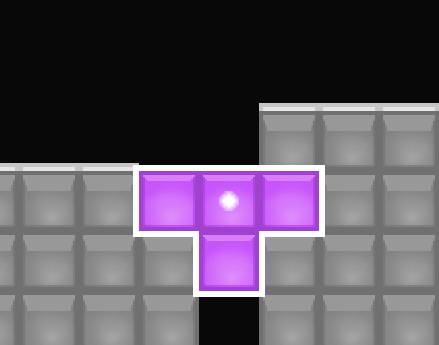
\includegraphics[width = 0.4 \textwidth]{img/2.png}
			\caption{A T-Spin Double.}
		\end{subfigure}
		\begin{subfigure}[b]{0.4\textwidth}
			\centering
			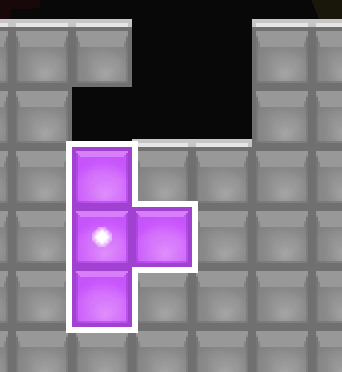
\includegraphics[width = 0.4 \textwidth]{img/3.png}
			\caption{A T-Spin Triple.}
		\end{subfigure}
		\caption{Some sample clears with SRS.}
	\end{figure}

	In Modern Tetris, human players often try to perform higher Attack Per Minute (APM), 
	but Tetris AI needs to perform higher Attack Per Piece (APP).
	
	To achieve a higher APP, we present KeroshiZeroTetris based on AlphaZero\cite{silver2018general}.

	However, directly applying the AlphaZero framework to Modern Tetris brings some difficulties:

	\begin{itemize}
		\item Unlike chess or Go, the next state is not fixed because of the 7-Bag random generator.
		\item The neural network for Modern Tetris must be carefully designed to predict both policy and value information.
		\item The Tetris AI needs to play indefinitely with a high APP,
			so a major challenge is how to set up training tasks and how to implement the trained policy in actual match play.
	\end{itemize}

	To solve these issues, this paper details the implementation of KeroshiZeroTetris.

	\section{Model}

	A Tetris model requires the following inputs:

	\begin{itemize}
		\item The board.
		\item The piece types of the current, hold and next queue.
		\item The values including Combo and Back-to-Back (B2B).
	\end{itemize}

	\begin{minipage}[t]{0.4\textwidth}
		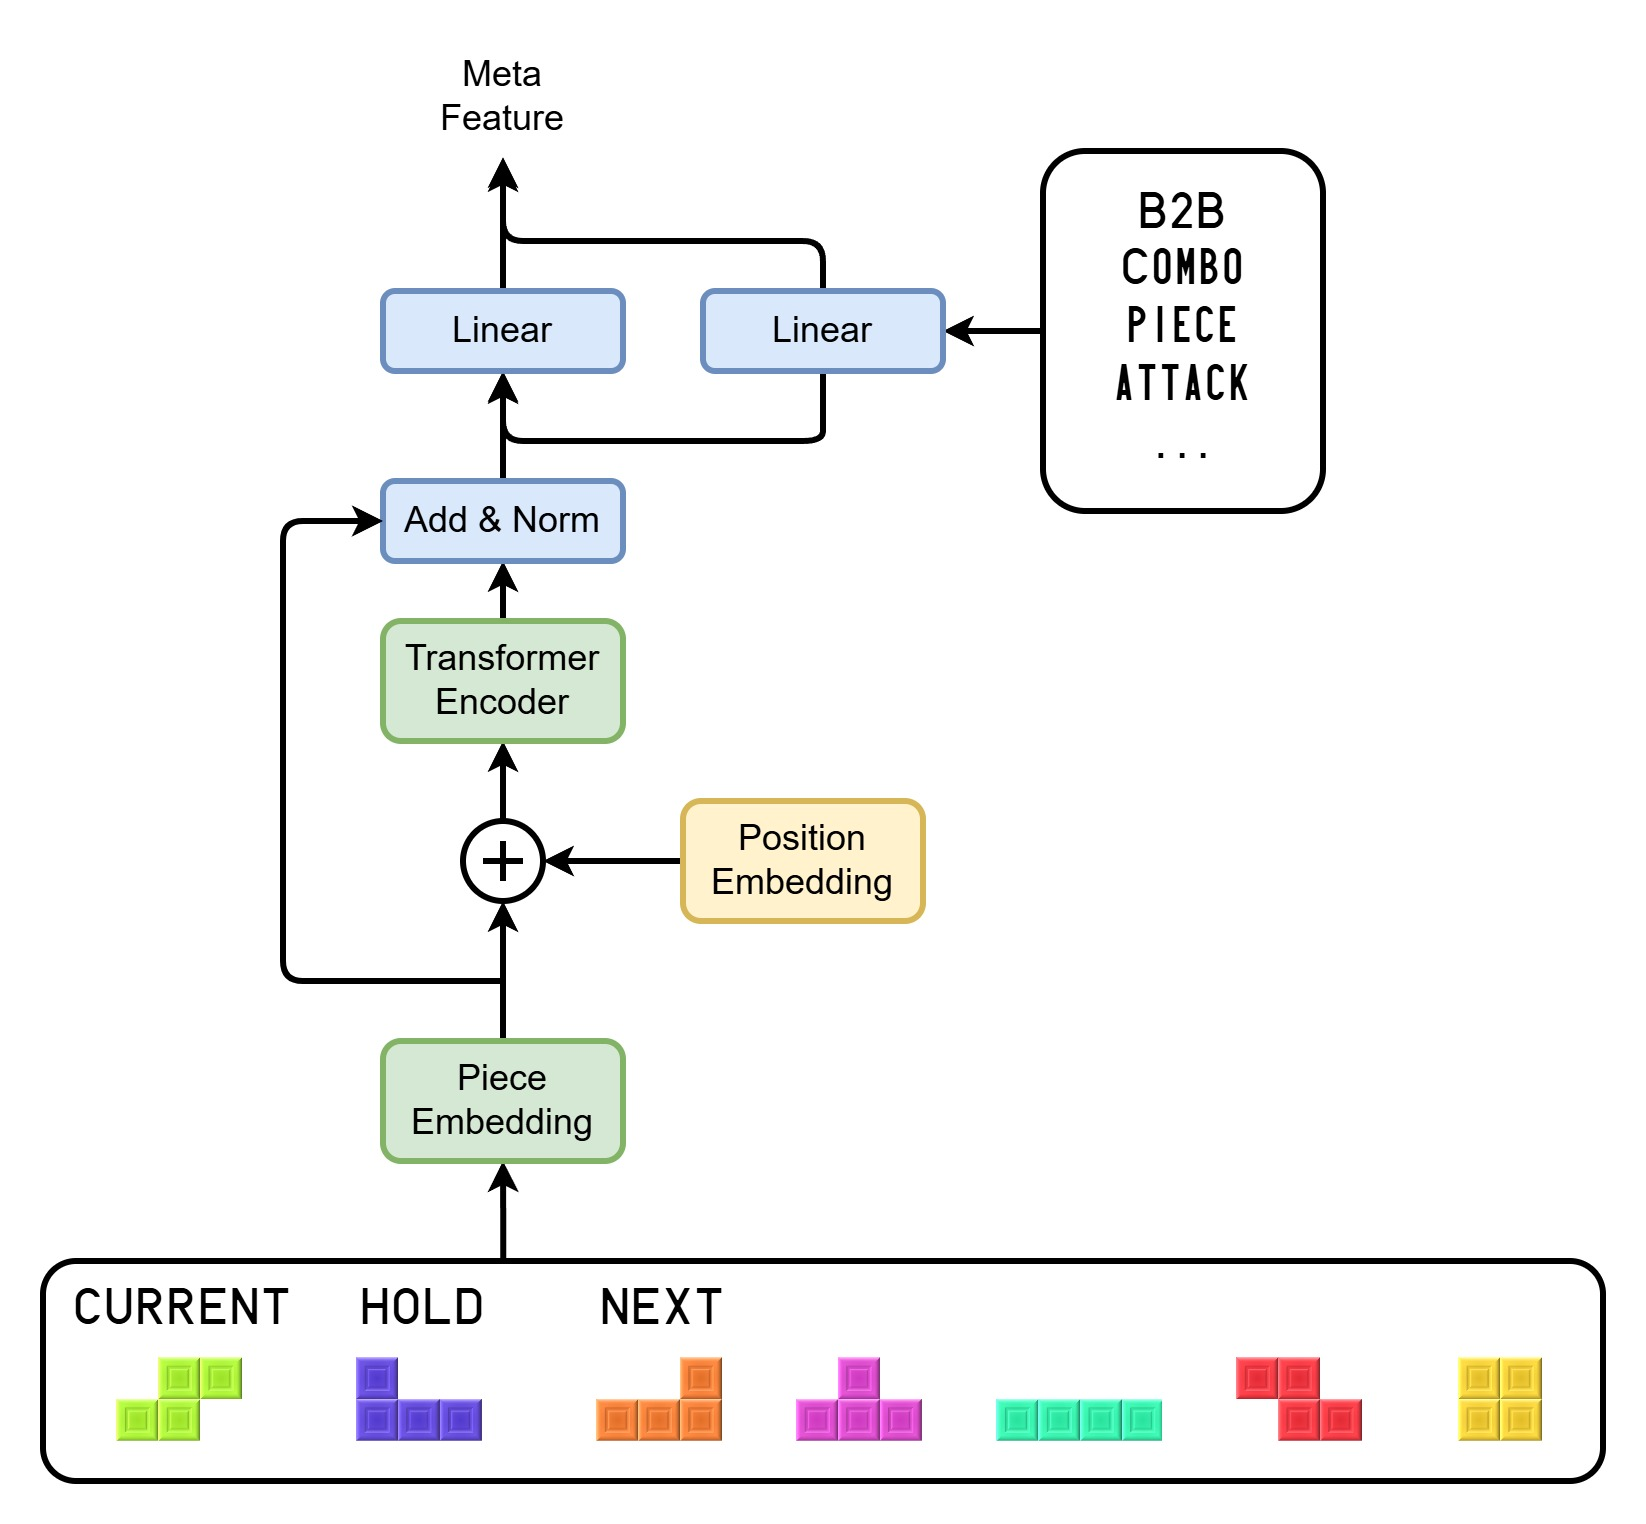
\includegraphics[width = \textwidth, align = t]{img/4.jpg}
		\captionof{figure}{The piece sequence encoder.}
	\end{minipage}
	\hfill
	\begin{minipage}[t]{0.55\textwidth}
		\hyphenpenalty = 10000

		\vspace{1em}

		We call the piece types the piece sequence.
		First we need to encode this sequence.

		First, we put the piece sequence into a Piece Embedding layer.
		Then we add the Position Embedding to it.
		After that, we send it into the Transformer Encoder\cite{vaswani2017attention}.
		To make the model converge faster, we bring the original piece sequence embedding to do a residual connection\cite{he2016deep}.
		Now, the piece sequence processing is finished.

		\vspace{1em}

		Next, we need to add the game data.
		We use a Linear layer on the game data first.
		Second, we join it with the sequence features and put them through another Linear layer.
		Finally, we join it with the processed game data from the first step.
		Now, the piece sequence and the game data are combined into a feature called Meta Feature.

	\end{minipage}

	\begin{minipage}[t]{0.3\textwidth}
		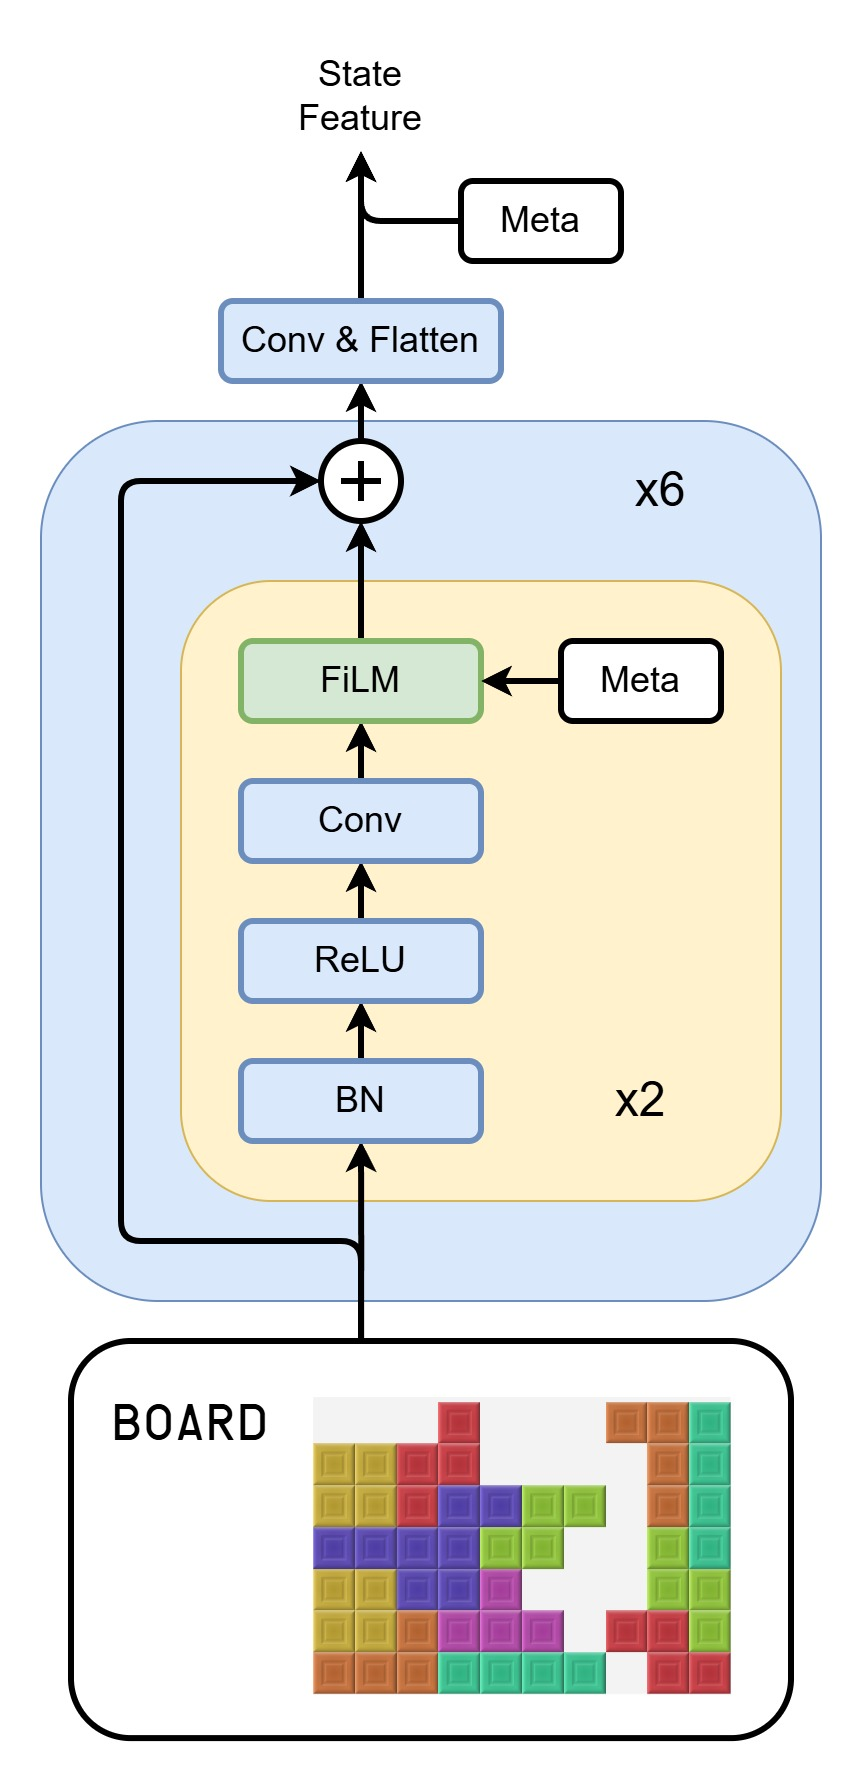
\includegraphics[width = \textwidth, align = t]{img/5.jpg}
		\captionof{figure}{The board encoder.}
	\end{minipage}
	\hfill
	\begin{minipage}[t]{0.65\textwidth}
		\hyphenpenalty = 10000

		\vspace{2em}
		After we process the piece sequence and game data, we need to mix them into the board.
		To do this, we use the FiLM\cite{perez2018film},
		and use the Meta feature as the condition.
		In the CNN part for the board, we use residual connections\cite{he2016deep} and pre-activation\cite{he2016identity}.
		Finally we use a Convolution layer and a Flatten layer.
		Then we combine the output with the original Meta Feature to get the final State Feature.

		Just like AlphaZero\cite{silver2018general},
		we use some Linear layers to connect the State Feature to Value Head and Policy Head.

		\vspace{1em}

		These are the detailed parameters of our model.

		\vspace{1em}

		\begin{tabular}{ll}
		\hline
		\textbf{Component} & \textbf{Size / Number} \\
		\hline

		Board Input						& $30 \times 10$ \\
		Piece Sequence Length			& $10$ \\
		Game Values						& $10$ \\

		\hline

		Piece Embedding Dimension		& $16$ \\
		Transformer Encoder Layers		& $1$ \\
		Meta Feature Dimension			& $256$ \\

		\hline

		CNN Channels					& $64$ \\
		Residual Blocks					& $6$ \\
		Flattened Board Feature			& $1200$ \\

		\hline

		State Feature Dimension			& $1456$ \\
		Value Head						& $1456 \rightarrow 256 \rightarrow 1$ \\
		Policy Head						& $1456 \rightarrow 512 \rightarrow 1537$ \\

		\hline
	\end{tabular}

	\end{minipage}


	\bibliographystyle{unsrt} 
	\bibliography{references}

\end{document}
